% !TEX root = ../main.tex
% !TEX program = xelatex
\section{问题二的模型建立与求解}

\subsection{求解思路}

问题一是在已知代表日供需曲线的情况下安排购电，而问题二要求每天0:00提前制定当天计划，此时当天真实负载和光伏尚未发生。普通电买少了，实际缺口需要按照正常电价的5倍紧急补购；买多了，若无法使用或储存，也仍需支付普通购电费用。因此，本问需要在\textbf{提前购电成本与紧急购电风险之间进行权衡}。

为此，本文依次比较三类方案：首先利用历史同期数据预测负载和光伏；其次引入岭回归和提升树，考察更复杂的预测方法能否降低实际费用；最后在历史预测基础上加入误差准备，针对供需缺口被低估后可能产生的高价紧急购电进行防范。

需要强调的是，本问的最终目标并不是使预测误差最小，而是使普通购电费用与紧急购电费用之和尽可能低。同样大小的预测误差，如果发生在不同电价或不同储电状态下，其经济影响可能完全不同。

因此，本文最终采用“历史分项预测--近期加权准备--跨日线性规划模型”。模型首先分别估计负载和光伏，再根据近期预测误差增加适量准备，随后利用线性规划制定普通购电计划。白天普通订单保持不变，储能设备根据实际供需补充缺口或吸收余电，剩余缺口才通过紧急购电补足。


\subsection{负载与光伏预测}

前文探索性分析表明，负载具有较明显的周重复特征，而光伏更适合参考近期发电水平。因此，本文不直接预测两者的差值，而是分别预测负载和光伏。

设$d$表示日期，$k=1,\ldots,144$表示日内第$k$个10分钟时段，每个时段长度为

\[
\Delta t=\frac{1}{6}\ \mathrm{h}.
\]

负载采用过去4个相同星期位置的同一时段平均，光伏采用最近7天同一时段的平均：

\begin{equation}
\widehat L_{d,k}
=
\frac{1}{4}\sum_{j=1}^{4}L_{d-7j,k},
\qquad
\widehat V_{d,k}
=
\frac{1}{7}\sum_{j=1}^{7}V_{d-j,k}.
\label{eq:q2_forecast}
\end{equation}

即负载主要利用周重复规律，光伏主要利用近期发电水平。历史记录不足时，只对当时已经存在的数据取平均。

为保证每天0:00制定计划时不使用未来信息，式\eqref{eq:q2_forecast}只使用当日零点以前已经发生的数据。虽然附件2保存了全年实际负载和光伏，但当天及之后的真实值均不参与当天预测；本问也不使用问题三才引入的附件3光伏预报。


\subsection{基于近期误差的准备量}

平均预测能够描述通常的供需水平，但如果连续低估负载或高估光伏，电池可能持续补充缺口并逐渐达到最低储电量。为降低这种风险，本文进一步利用近期预测误差确定购电准备量。

对历史日期$i$，定义第$k$个时段的净供需预测误差为

\begin{equation}
\varepsilon_{i,k}
=
\left[
(L_{i,k}-V_{i,k})
-
(\widehat L_{i,k}-\widehat V_{i,k})
\right]\Delta t .
\label{eq:q2_error}
\end{equation}

其中，$\varepsilon_{i,k}>0$表示实际供需缺口比预测值更大，即存在低估缺口的风险；负值则表示预测偏保守。

本文将一天划分为六个4小时区间，在最近28天内收集同一时间区间的误差。为使准备量更及时地反映近期变化，对较新的误差赋予更高权重：

\begin{equation}
\omega_{d,i,k}
=
\frac{\beta^{d-1-i}}
{\displaystyle
\sum_{(j,u)\in E_{d,g}}
\beta^{d-1-j}},
\qquad
(i,k)\in E_{d,g},
\label{eq:q2_weight}
\end{equation}

其中，$E_{d,g}$表示最近28天中第$g$个4小时区间的历史误差集合，$\beta$为时间衰减参数。

随后将误差从小到大排列，取加权累计比例达到$\alpha$的位置作为准备依据，并将负值截为0：

\begin{equation}
F_{d,g}(u)
=
\sum_{(i,k)\in E_{d,g}}
\omega_{d,i,k}
\mathbf{1}
\left(
\varepsilon_{i,k}\leq u
\right),
\label{eq:q2_cdf}
\end{equation}

\begin{equation}
b_{d,k}
=
\max
\left\{
0,\,
\inf
\left[
u:F_{d,g(k)}(u)\geq\alpha
\right]
\right\}.
\label{eq:q2_reserve}
\end{equation}

本文取

\[
\alpha=0.7,\qquad \beta=0.7.
\]

其中，$\alpha$控制准备程度，$\beta$控制历史误差随时间的衰减速度，两者含义不同。准备量$b_{d,k}$被加入预测净需求，由后续优化模型统一安排，并不意味着每个时段直接多购买固定数量的电。

为避免参数选择与最终全年评价混用，本文将两者分开处理：参数在前期历史数据比较中确定，2--12月的完整运行结果用于最终评价和灵敏度检验，而不再反向调整模型参数。


\subsection{购电与储能优化模型}

\subsubsection*{（1）决策变量与预测净需求}

为减弱单日末端边界对储能决策的影响，每天0:00向前规划48小时，共288个10分钟时段，但只固定当天前144个时段的普通购电计划。

也就是说，模型会考虑午夜以后仍可能存在的用电需求，但不会提前锁定第二天的正式普通购电订单。
根据预测负载、光伏和准备量，定义规划期内第$t$个时段的预测净需求为

\begin{equation}
r_t
=
(\widehat L_t-\widehat V_t)\Delta t+b_t,
\label{eq:q2_net_demand}
\end{equation}

并令

\[
n_t=\max(r_t,0),
\qquad
a_t=\max(-r_t,0),
\]

其中，$n_t$表示预计需要由外网或储能补充的电量，$a_t$表示预计可以用于储能的富余电量。

设置以下连续决策变量：

\[
x_t:\text{外网购电中用于储能充电的电量},
\]

\[
y_t:\text{光伏富余中用于储能充电的电量},
\]

\[
z_t:\text{储能设备向负载输出的电量},
\]

\[
S_t:\text{时段结束时的内部储电量}.
\]

则普通计划购电量为

\begin{equation}
q_t=n_t-z_t+x_t.
\label{eq:q2_purchase}
\end{equation}

其含义是：预计负载缺口先由电池承担一部分，其余由外网补足；同时，模型也可以在合适的时段额外购电给电池充电。


\subsubsection*{（2）目标函数}

48小时规划期内按照固定日内电价计算普通计划费用。为避免模型在规划末端无意义地将储能完全放空，对期末剩余电量赋予参考价值：

\begin{equation}
\min J
=
\sum_{t=1}^{288}p_tq_t
-
\nu S_{288},
\qquad
\nu=0.9p_{00:00}.
\label{eq:q2_objective}
\end{equation}

其中，该期末价值仅用于比较规划方案，并不表示电池可以向外网售电，也不从最终实际购电费用中扣除。


\subsubsection*{（3）约束条件}

为保证购电计划满足储能设备的实际运行要求，设置以下约束。

\textbf{1）储电量递推约束}

储能设备的充电效率和放电效率均为90\%。因此，第$t$个时段结束后的内部储电量为

\begin{equation}
S_t
=
S_{t-1}
+
0.9(x_t+y_t)
-
\frac{z_t}{0.9}.
\label{eq:q2_soc}
\end{equation}

其中，$x_t+y_t$表示进入储能设备的外侧充电量，$z_t$表示储能设备实际向负载输出的电量。充入100 kWh电量时，内部储电量增加90 kWh；向负载输出90 kWh时，内部储电量减少100 kWh。


\textbf{2）储电容量约束}

为避免储能设备过度充电或放电，内部储电量必须保持在允许范围内：

\begin{equation}
1200
\leq
S_t
\leq
10800.
\label{eq:q2_soc_bound}
\end{equation}

该约束保证储能设备始终处于题目规定的安全运行区间。


\textbf{3）充电约束}

外网充电量$x_t$不得为负，光伏充电量$y_t$不能超过该时段预计的光伏富余量$a_t$：

\begin{equation}
x_t\geq0,
\qquad
0\leq y_t\leq a_t.
\label{eq:q2_charge_source}
\end{equation}

储能最大充电功率为5000 kW，每个调度时段为10分钟，因此单个时段的总充电量满足

\begin{equation}
x_t+y_t
\leq
5000\Delta t
=
833.33\ \mathrm{kWh}.
\label{eq:q2_charge_limit}
\end{equation}


\textbf{4）放电约束}

储能放电量不能超过该时段的预计负载缺口$n_t$，同时受到最大放电功率限制：

\begin{equation}
0
\leq
z_t
\leq
\min
\left\{
n_t,\,
5000\Delta t
\right\}.
\label{eq:q2_discharge_limit}
\end{equation}

该约束避免储能向负载提供超过实际需求的电量，也保证放电功率不超过设备上限。


\textbf{5）普通购电非负约束}

各时段的普通计划购电量不能为负：

\begin{equation}
q_t\geq0.
\label{eq:q2_purchase_nonnegative}
\end{equation}


\textbf{6）初始储电状态约束}

每天进行48小时滚动规划时，规划起点的储电量取当天0:00实际剩余的电量：

\begin{equation}
S_0=S_{d,0}.
\label{eq:q2_initial_soc}
\end{equation}

问题二不再要求每天0:00与24:00的储电量相同。当天实际运行结束后的储电量继续作为下一天的初始状态，从而保持储能设备在全年运行过程中的连续性。


\subsection{日内实际供电与跨日运行}

每天0:00完成预测、误差准备和线性规划后，得到当天144个时段的普通购电订单。白天普通订单保持不变，但储能充放电可以根据已经发生的真实负载和光伏进行调整。

运行时首先由光伏直接满足负载。设某时段实际负载电量和光伏电量分别为$l$和$v$，则光伏直供后剩余负载记为$h$。

若实际剩余负载超过普通购电量，则优先由电池在储电量和放电功率允许范围内补充，剩余部分才进行紧急购电：

\begin{equation}
z
=
\min
\left\{
h-q,\,
5000\Delta t,\,
0.9(S-1200)
\right\},
\qquad
e=h-q-z.
\label{eq:q2_emergency}
\end{equation}

其中，$e$为紧急购电量。即使电池仍有存量，若已经接近1200 kWh下限或受到5000 kW放电功率限制，也可能无法完全补足当前缺口。

若普通购电已经能够覆盖实际剩余负载，则优先将实际光伏富余和普通购电余量用于储能充电，并受到储能容量和充电功率限制。

因此，第$d$天实际购电费用为

\begin{equation}
C_d
=
\sum_{k=1}^{144}
\left(
p_kq_{d,k}
+
5p_ke_{d,k}
\right),
\label{eq:q2_daily_cost}
\end{equation}

并满足跨日状态传递

\begin{equation}
S_{d+1,0}=S_{d,144}.
\label{eq:q2_cross_day}
\end{equation}

由此，每天在零点制定计划，日内先用储能吸收偏差，必要时紧急购电，
再将剩余库存传递至下一天，形成连续的调度过程。

全年运行从2025年1月1日0:00的6000 kWh开始。首日没有更早历史，因此采用问题一得到的购电安排启动。随后利用逐日积累的历史数据滚动更新预测和准备量。1月份用于完成启动及参数选择，2月1日起进入题目要求的正式统计范围；此时储电量由1月份连续运行承接，而不是重新设置为6000 kWh。


\subsection{参数依据与方案比较}

模型选择时，以最终实际购电费用作为主要评价标准。预测误差较小通常有利，但同样大小的误差若出现在高价时段，或连续消耗储能库存，仍可能造成较高紧急购电费用。

因此，本文比较了历史分项预测、岭回归、提升树以及加入误差准备后的多种方案。各方案使用相同的电价、储能设备、起始状态、规划长度和实际供电规则。

预测窗口通过前期数据比较确定为负载4周、光伏7天，并取$\alpha=0.7$、$\beta=0.7$。

其中，岭回归和提升树主要以提高预测精度为目标，并未直接考虑预测误差在不同电价与储能状态下造成的经济损失。因此，预测误差较小并不一定意味着最终购电费用更低。相比之下，近期加权准备直接针对缺口低估可能引起的高价紧急购电风险。

2月1日至12月31日334天的实际费用比较如表\ref{tab:q2_model_compare}所示。

\begin{table}[htbp]
\centering
\caption{不同方案的334天实际购电费用}
\label{tab:q2_model_compare}
\begin{tabular}{lccc}
\hline
方案 & 普通电费/万元 & 紧急电费/万元 & 总电费/万元 \\
\hline
历史分别预测，无误差准备
& 1218.58 & 374.70 & 1593.28 \\
分别岭回归，无误差准备
& 1210.27 & 446.88 & 1657.15 \\
分别提升树，无误差准备
& 1218.25 & 343.71 & 1561.96 \\
历史分别预测，等权误差准备
& 1295.99 & 107.05 & 1403.04 \\
历史分别预测，近期加权准备
& \textbf{1297.96} & \textbf{60.43} & \textbf{1358.38} \\
\hline
\end{tabular}
\end{table}

近期加权准备方案的普通电费比等权准备方案增加约1.97万元，但紧急电费减少约46.63万元，因此总费用减少约44.66万元，降幅为3.18\%。与不设置误差准备的历史预测方案相比，总费用下降约14.74\%。

提升树虽然降低了部分预测误差，却没有取得最低的实际购电费用。这进一步说明，本问应围绕最终经济成本选择方案，而不能仅以预测精度决定模型优劣。

因此，候选方案的实际费用比较支持了本文采用“历史分项预测--近期加权准备--跨日线性规划”的结构，但该比较仅针对已实际测试的模型与参数组合，不表示已经排除了所有其他预测方法。


\subsection{全年结果与指定日期分析}

2025年2月1日至12月31日共334天，最终方案总费用为

\[
\boxed{13583810.84\ \text{元}},
\]

其中普通购电费用为

\[
12979560.57\ \text{元},
\]

紧急购电费用为

\[
604250.27\ \text{元}.
\]

完整10分钟结果保存于\texttt{result2.xlsx}。


\subsubsection*{（1）月度费用分析}

图\ref{fig:q2_monthly_cost}给出了各月普通购电费、紧急购电费，以及近期加权方案相对于等权准备方案的节省金额。

\begin{figure}[htbp]
    \centering
    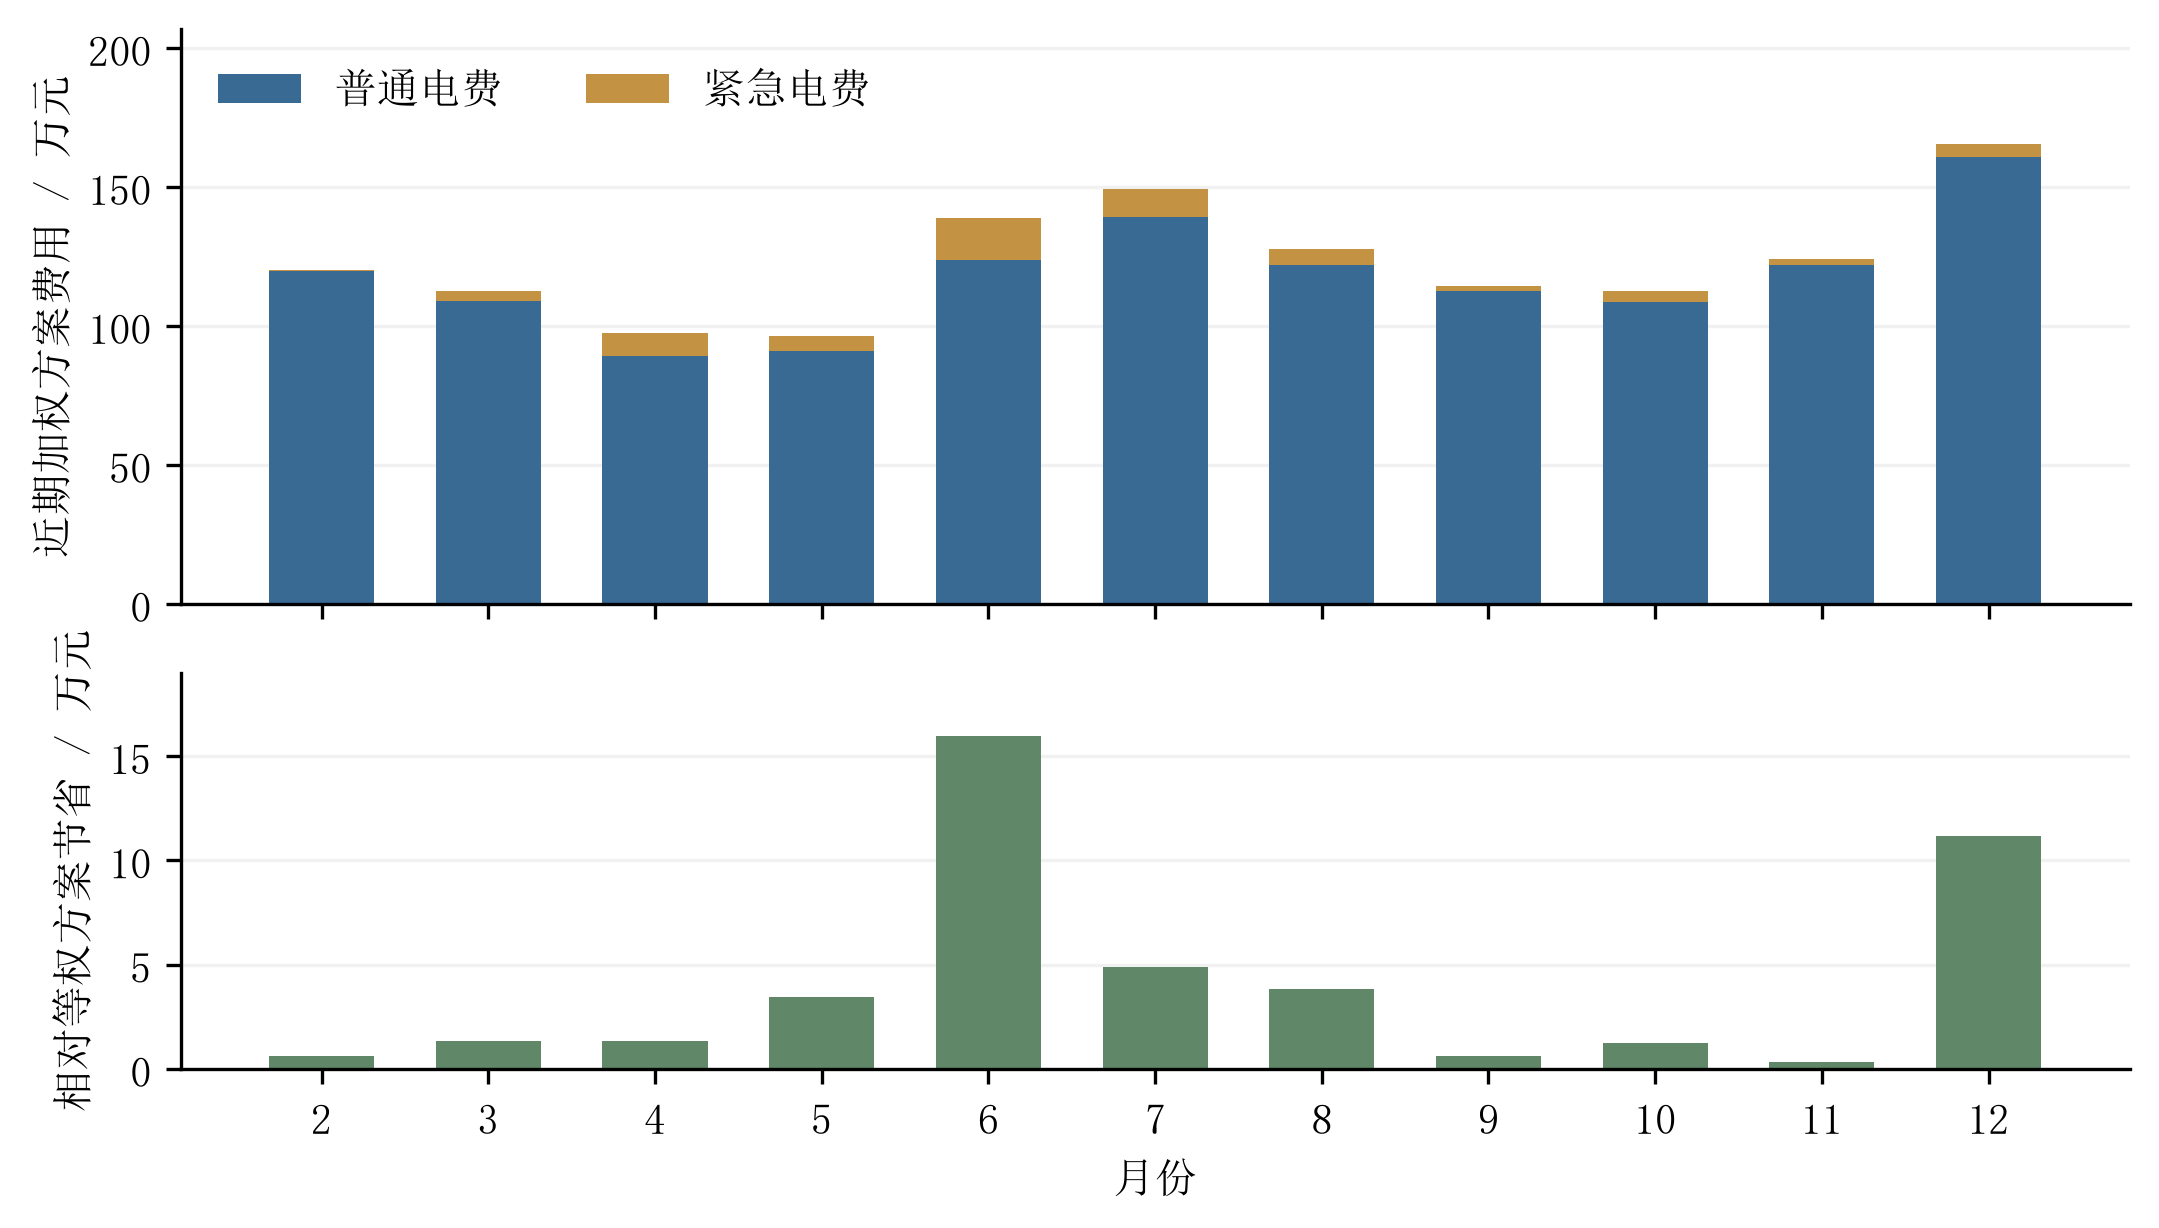
\includegraphics[width=0.95\textwidth]{fig/monthly_cost.png}
    \caption{近期加权准备方案的月度费用及相对等权准备的节省}
    \label{fig:q2_monthly_cost}
\end{figure}

由图\ref{fig:q2_monthly_cost}可见，各月份费用主要由普通购电组成，但紧急购电由于价格较高，对总费用仍有明显影响。11个月合计均取得节省，其中6月和12月的贡献较大。

这说明近期误差能够为购电准备提供有效信息，但其效果会随着具体供需条件变化。逐日结果并不保证每一天都比等权方案更便宜，因此其优势应从全年总费用角度评价。


\subsubsection*{（2）指定日期购电结果}

题目指定四个日期的购电和费用结果如表\ref{tab:q2_specified_purchase}所示。

\begin{table}[H]
\centering
\caption{指定日期的计划购电及全天费用}
\label{tab:q2_specified_purchase}
\begin{tabular}{lrrrr}
\hline
项目 & 3月20日 & 6月21日 & 9月23日 & 12月21日 \\
\hline
10:00--10:10
& 0.00 & 0.00 & 0.00 & 0.00 \\
12:00--12:10
& 610.16 & 0.00 & 484.48 & 943.63 \\
14:00--14:10
& 0.00 & 0.00 & 0.00 & 0.00 \\
16:00--16:10
& 434.90 & 116.65 & 453.86 & 798.03 \\
18:00--18:10
& 716.29 & 437.88 & 826.38 & 742.86 \\
20:00--20:10
& 0.00 & 0.00 & 5.90 & 0.00 \\
全天计划购电量/kWh
& 64232.05 & 40298.69 & 68385.07 & 95446.27 \\
全天紧急购电量/kWh
& 329.52 & 0.00 & 6.38 & 0.00 \\
全天购电合计/kWh
& 64561.57 & 40298.69 & 68391.44 & 95446.27 \\
普通电费/元
& 39469.74 & 22323.80 & 42730.05 & 61249.77 \\
紧急电费/元
& 2298.74 & 0.00 & 43.00 & 0.00 \\
总电费/元
& 41768.47 & 22323.80 & 42773.04 & 61249.77 \\
\hline
\end{tabular}
\end{table}

各日全天结果均由完整144个10分钟区间汇总得到，不能由表中展示的六个指定时段直接相加得到。


\subsubsection*{（3）指定日期储能运行结果}

各指定日期的实际充放电情况如表\ref{tab:q2_storage}所示。

\begin{table}[H]
\centering
\caption{指定日期的实际充放电量及日首尾储电量}
\label{tab:q2_storage}
\begin{tabular}{llrrrr}
\hline
时间段 & 项目 & 3月20日 & 6月21日 & 9月23日 & 12月21日 \\
\hline
00:00--04:00 & 充电
& 1504.96 & 309.75 & 1739.22 & 1830.47 \\
& 放电
& 185.93 & 229.12 & 2.78 & 227.55 \\

04:00--08:00 & 充电
& 1138.95 & 286.60 & 53.65 & 1476.38 \\
& 放电
& 4670.35 & 1949.50 & 5934.88 & 729.24 \\

08:00--12:00 & 充电
& 5327.26 & 10134.27 & 4409.06 & 4706.14 \\
& 放电
& 3265.56 & 0.00 & 2387.94 & 8254.51 \\

12:00--16:00 & 充电
& 4465.10 & 21.43 & 6147.58 & 8347.54 \\
& 放电
& 369.53 & 0.00 & 521.04 & 2318.98 \\

16:00--20:00 & 充电
& 169.64 & 115.05 & 221.91 & 19.45 \\
& 放电
& 5340.10 & 5107.80 & 4920.36 & 4873.96 \\

20:00--24:00 & 充电
& 4438.27 & 8636.77 & 8446.30 & 8360.50 \\
& 放电
& 3424.22 & 3022.72 & 3633.41 & 3626.10 \\
\hline
0:00储电量/kWh & 
& 8919.73 & 3543.84 & 9214.11 & 8886.94 \\
24:00储电量/kWh &
& 5086.49 & 9642.73 & 8796.25 & 8897.44 \\
\hline
\end{tabular}
\end{table}

表中的充、放电量按储能设备外侧计量，日初和日末储电量按内部电量计量。一个4小时区间内同时存在充电量和放电量，仅表示不同10分钟时段执行了不同动作，并非同一时段同时充放电。


\subsubsection*{（4）指定日期紧急购电}

按照赛题要求的表格形式，将四个指定日期的紧急购电结果整理如表\ref{tab:q2_emergency_purchase}所示。

% Restored from verified Q2 selected_execution.csv.gz; no model rerun.
\begin{table}[H]
\centering
\caption{问题二指定日期发生紧急购电的时段及电量}
\label{tab:q2_emergency_purchase}
\begin{tabular}{llr}
\toprule
日期 & 时间段 & 紧急购电量/kWh \\
\midrule
3月20日 & 20:40--20:50 & 329.52 \\
9月23日 & 20:30--20:40 & 6.38 \\
\bottomrule
\end{tabular}
\end{table}


四个指定日期中，3月20日和9月23日发生紧急购电，6月21日和12月21日均未发生紧急补购。


\subsubsection*{（5）储能对预测偏差的缓冲作用}

为进一步解释紧急购电产生的原因，图\ref{fig:q2_specified_days}选取3月20日和6月21日进行比较。

\begin{figure}[H]
    \centering
    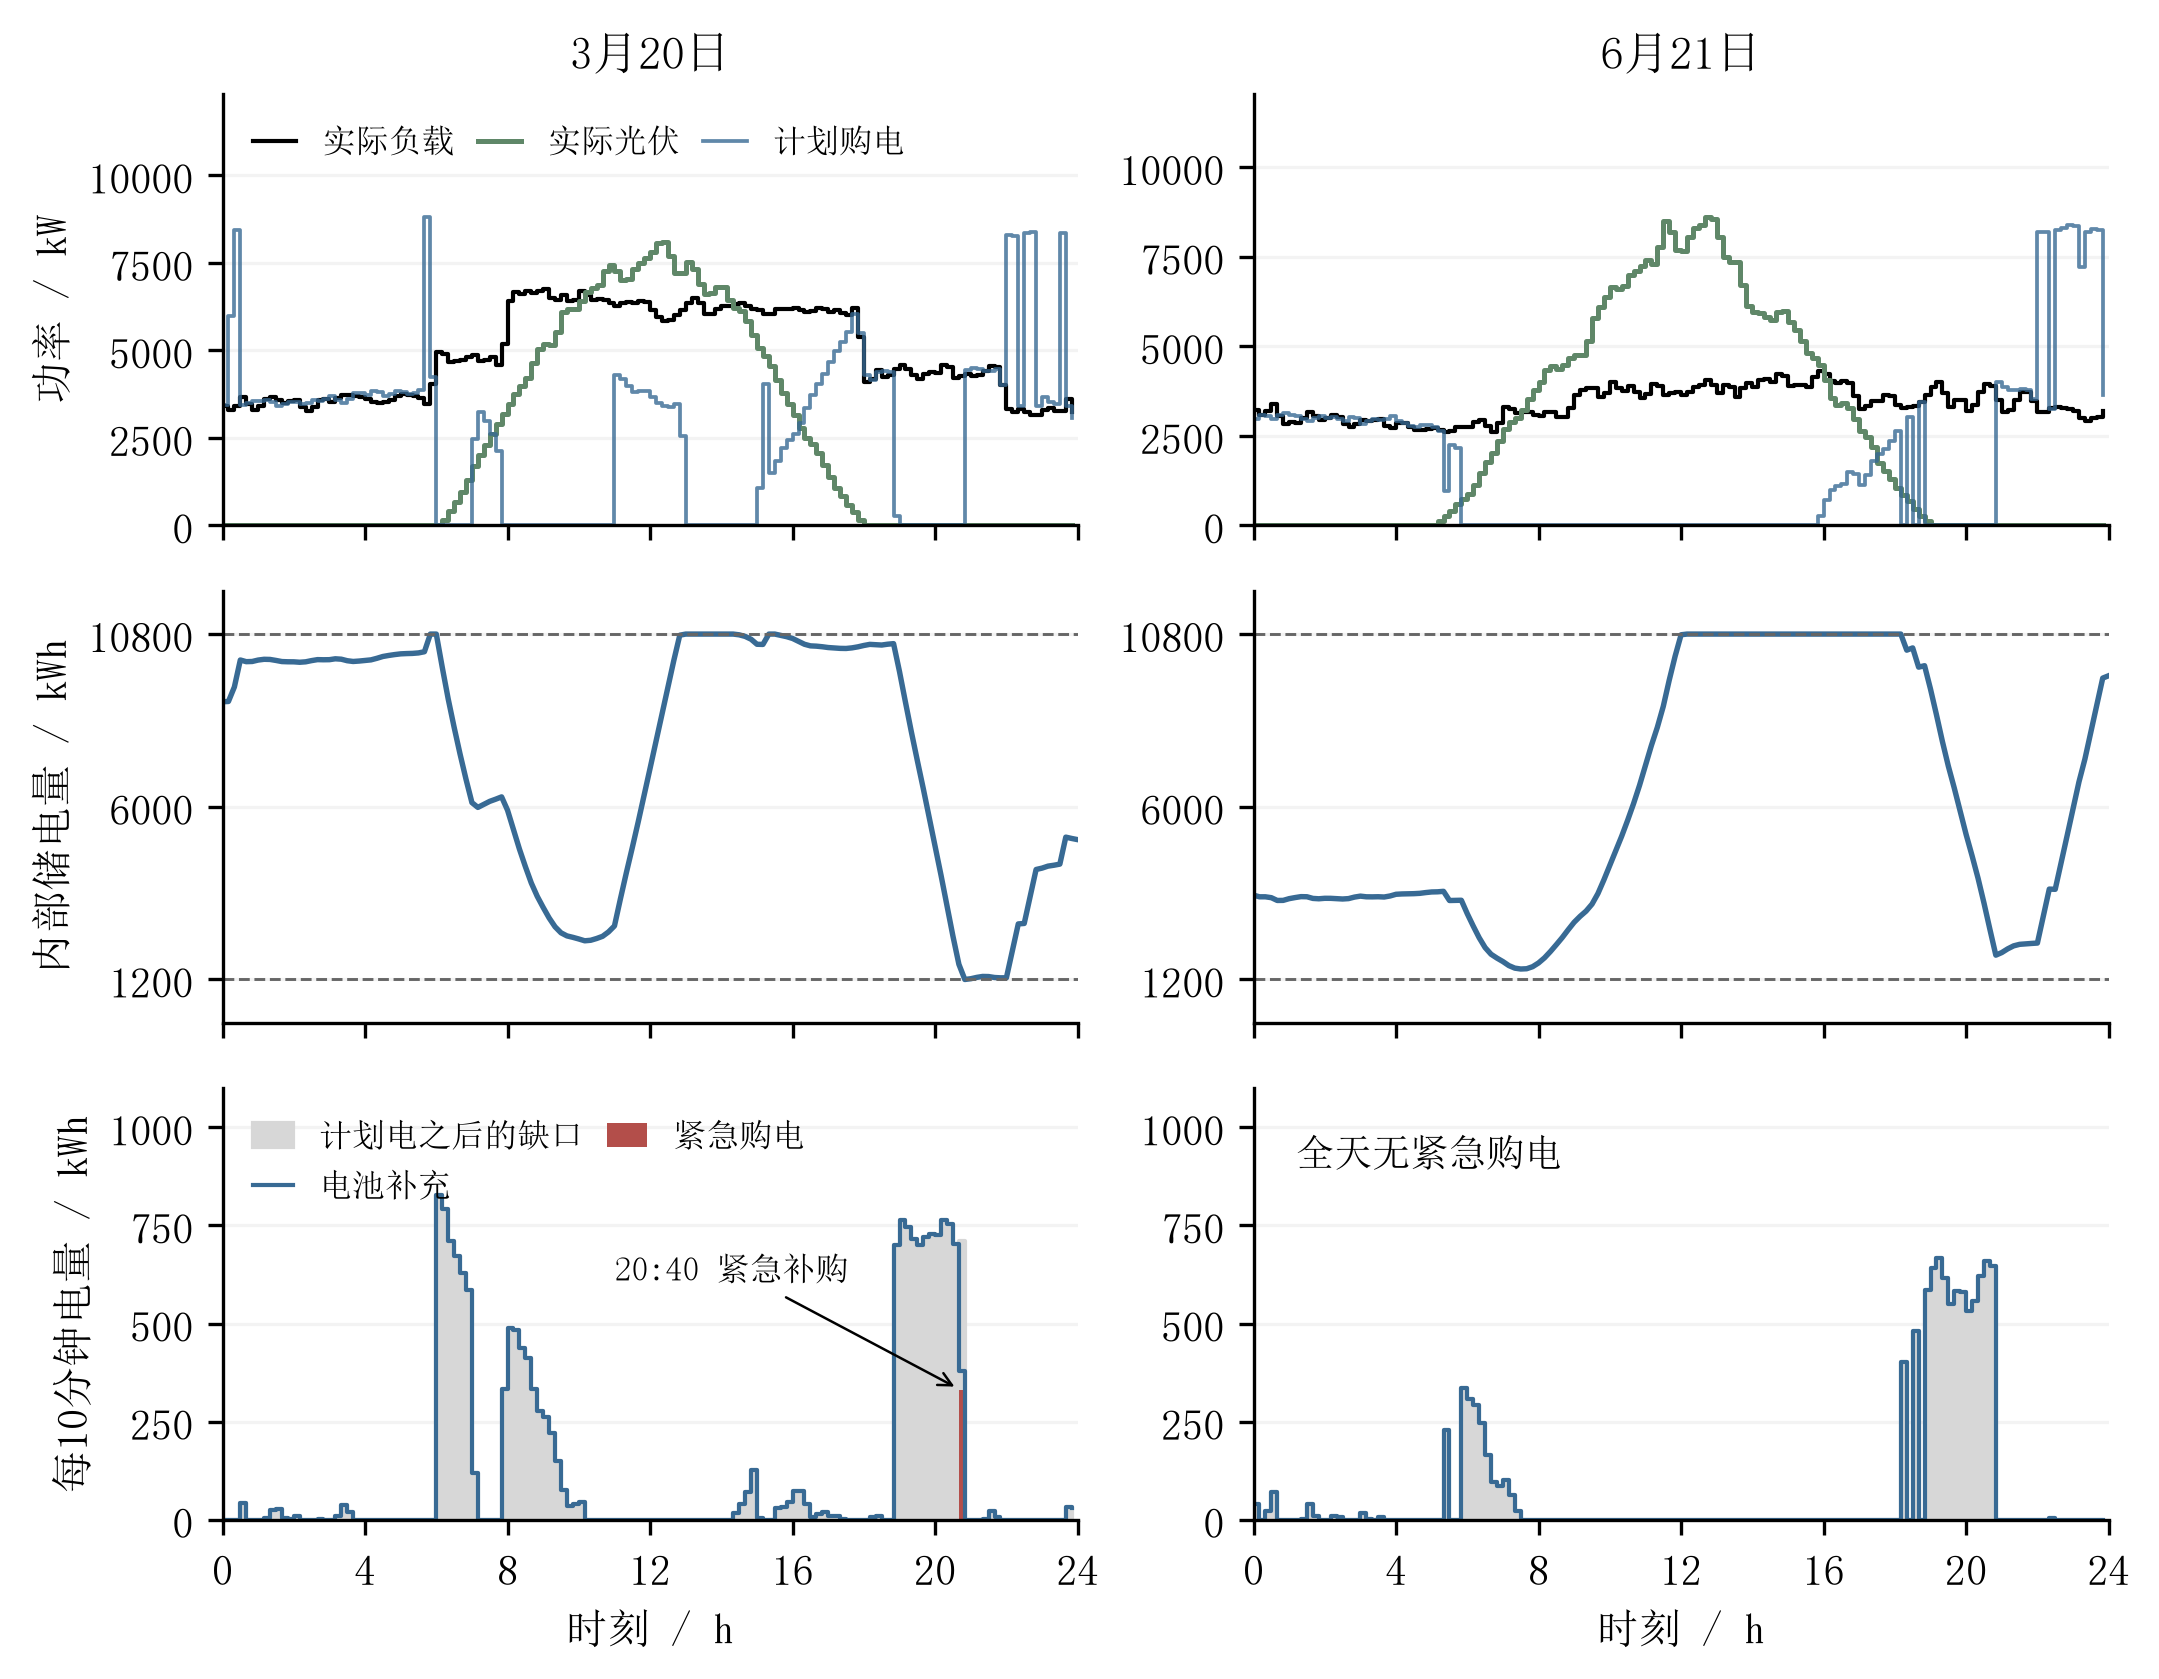
\includegraphics[width=\textwidth]{fig/specified_days.png}
    \caption{两个指定日期的供需、储电量与缺口补充情况}
    \label{fig:q2_specified_days}
\end{figure}

3月20日的大部分供需缺口都能够由储能设备补充，但20:40开始时内部储电量仅剩1622.06 kWh。继续放电后达到1200 kWh下限，因此仍有329.52 kWh的缺口只能通过紧急购电补足。

相比之下，6月21日白天实际光伏较多，储能能够吸收光伏并在后续时段释放，因此全天没有发生紧急购电。

由图\ref{fig:q2_specified_days}可以看出，判断是否需要紧急购电，不能只比较全天总供需量，而应同时考虑\textbf{缺口发生的时刻、当时剩余储电量以及储能的最大放电能力}。


\subsection{灵敏度检验与风险分析}

为考察准备量参数对最终费用的影响，分别改变分位参数$\alpha$和时间衰减参数$\beta$，其余条件保持不变，并以

\[
\alpha=\beta=0.7
\]

作为基准。

图\ref{fig:q2_sensitivity}给出了不同参数下普通电费、紧急电费和总费用的变化。

\begin{figure}[H]
    \centering
    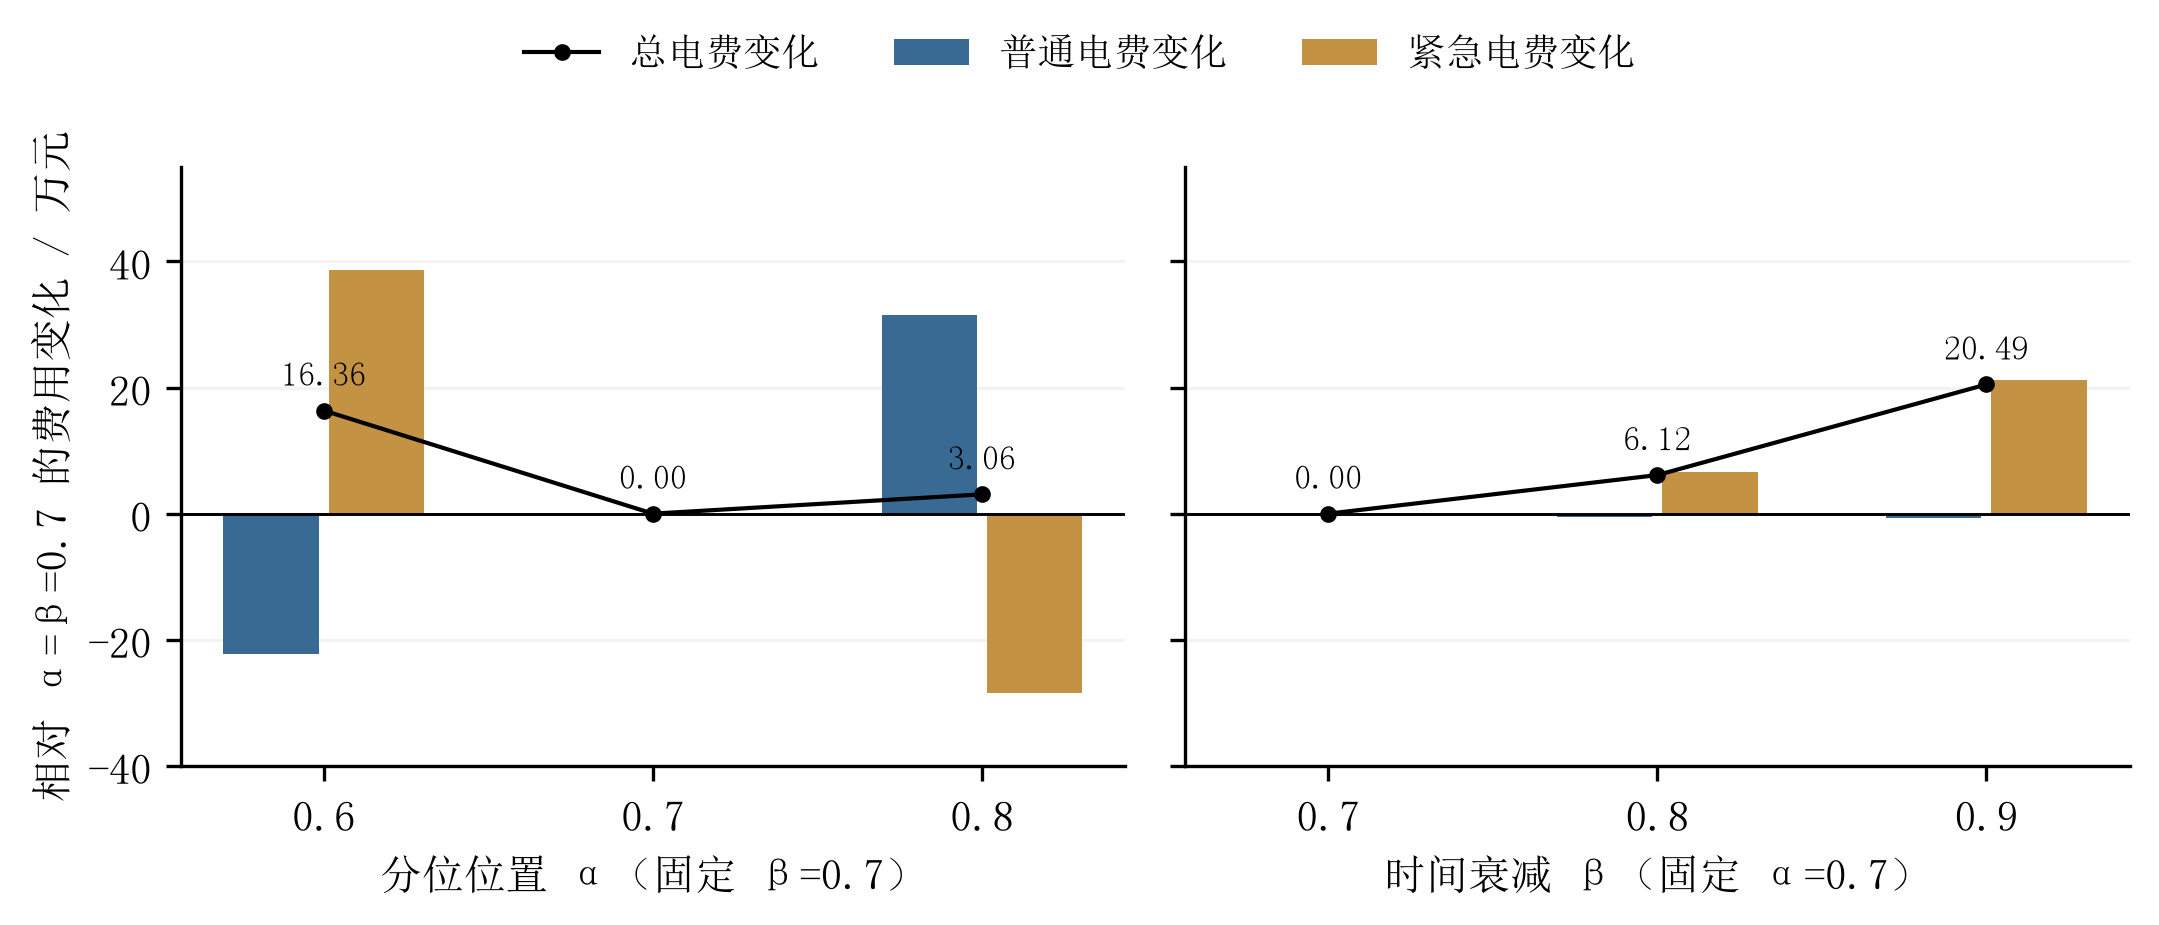
\includegraphics[width=0.95\textwidth]{fig/sensitivity.png}
    \caption{准备程度与近期权重对购电费用的影响}
    \label{fig:q2_sensitivity}
\end{figure}

当固定$\beta=0.7$时，将$\alpha$提高到0.8后，紧急购电天数由156天减少至102天，但普通购电费用的增加超过紧急购电费用的下降，使总费用反而增加约3.06万元；当$\alpha$降至0.6时，准备不足使总费用增加约16.36万元。

当固定$\alpha=0.7$时，将$\beta$提高到0.8和0.9，总费用分别增加约6.12万元和20.49万元。较大的$\beta$使旧误差保留更高权重，从而降低准备量对近期供需变化的响应速度。

因此，\textbf{准备程度并不是越高越好}。准备不足会增加昂贵的紧急购电，而准备过多又会提高普通购电成本。在本文实际检验的参数范围内，$\alpha=\beta=0.7$的综合费用较低，但不能据此认为其是所有连续参数取值中的唯一最优解。

进一步逐段检查表明，最终方案仍有部分日期发生紧急购电。这并不意味着模型失效，而是说明储能设备只能在其容量和功率范围内缓冲预测误差；当电池已经达到最低库存或受到放电功率限制时，紧急购电仍不可避免。

已有连续偏差情景检验中，近期加权方案相对于等权准备仍保持一定费用优势，但该结果仅基于本题一个年份及有限情景，因此只能说明模型在当前数据条件下具有一定稳定性，不能直接推广到其他年份或其他微网。
